As introduced in \autoref{sec:intro-external-nondet}, the environment might
affect the transmission of messages, so called external nondeterminism.  The
tester should take the environment into account when validating its
observations.

This section explains how to address external nondeterminism by specifying the
environment, using the networked server example.  It corresponds to the
``Composition'' arrow in \autoref{fig:framework}.  \autoref{sec:net-tcp} defines
a model for concurrent TCP connections.  \autoref{sec:net-compose} then composes
the network model with the server specification, yielding a tester-side
specification that defines the space of valid observations.

\subsection{Modelling the network}
\label{sec:net-tcp}
When testing servers over the network, request and response packets may be
delayed.  As a result, messages from one end might arrive at the
other end in a different order from that they were sent.

The space of network reorderings can be modelled by a {\em network model}, a
conceptual program for the ``network wire''.  The wire can be viewed as a
buffer, which absorbs packets\footnote{In this section, ``packet'' is a
shorthand for the ``symbolic packet'' defined on
Page~\pageref{def:symbolic-packet}.} and later emits them:
\begin{coq}
  Notation packet := symbolic_packet.

  Definition netE: Type -> Type :=
    ioE packet packet.

  Notation Absorb := Recv.
  Notation Emit   := Send.
\end{coq}

For example, the network model for concurrent TCP connections is defined in
\autoref{fig:tcp-model}.  The model captures TCP's feature of maintaining the
order within each connection, but packets in different connections might be
reordered arbitrarily.  When the wire chooses a packet to send, the candidate
must be the oldest in its connection.

\begin{figure}
\begin{coq}
(* filter the oldest packet in each connection *)
Context oldest_in_each_conn : list packet -> list packet.

Fixpoint pick_one (l: list packet) : itree nondetE (option packet) :=%\label{def:pick-one}%
  if l is p::l'
  then or (Ret (Some p)) (pick_one l')
  else ret None.

CoFixpoint tcp (buffer: list packet) : itree (netE +' nondetE) void :=
  let absorb := pkt <- trigger Absorb;;
                tcp (buffer ++ [pkt])      in
  let emit p := trigger (Emit p);;
                tcp (remove pkt buffer)    in
  let pkts   := oldest_in_each_conn buffer in
  opkt <- pick_one pkts;;
  if opkt is Some pkt
  then emit pkt
  else absorb.
\end{coq}
\vspace*{1em}
\caption[Network model for concurrent TCP connections.]{Network model for
  concurrent TCP connections.  The model is an infinite program iterating over a
  \ilc{buffer} of all packets en route.  In each iteration, the model either
  \ilc{absorb}s or \ilc{emit}s some packet, depending on the current
  \ilc{buffer} state and the choice made in \ilc{pick_one}.  Any absorbed packet
  is appended to the end of buffer.  When emitting a packet, the model may
  choose a connection and send the oldest packet in it.}
\label{fig:tcp-model}
\end{figure}

Note the \ilc{pick_one} function, which might return (i) \ilc{Some p} or (ii)
\ilc{None}.  The network model then (i) emits packet \ilc p or (ii) absorbs a
packet into \ilc{buffer}.

\begin{itemize}
\item When the given list \ilc{pkts} is empty, \ilc{pick_one} always returns
  \ilc{None}, because the wire has no packet in the \ilc{buffer}, and must
  absorb some packet before emitting anything.
\item Given a non-empty linked list \ilc{(p::l')}, with \ilc p as head and
  \ilc{l'} as tail, \ilc{pick_one} might return \ilc{(Some p)} by choosing the
  left branch.  In this case, the wire can emit packet \ilc p.  Or the function
  might choose the right branch and recursing on \ilc{l'}, meaning that the wire
  can emit some packet in \ilc{l'} or absorb some packet into the buffer.
\end{itemize}

This network model reflects the TCP environment, where messages are never lost
but might be indefinitely delayed.  In the next subsection, I'll demonstrate how
to compose the server and network models into a client-side observation model.

\subsection{Network composition}
\label{sec:net-compose}

The network connects the server on one end to the clients on other ends.  When
one end sends some message, the network model absorbs it and later emits it to
the destination.

To {\em compose} a server model with a network model is to pair the server's
\ilc{Send} and \ilc{Recv} events with the network's \ilc{Absorb} and \ilc{Emit}
events.  Since the network model is nondeterministic, it might not be ready at
some given moment to absorb packets sent by the server.  The network might also
emit a packet before the server is ready to receive it.

\begin{figure}
  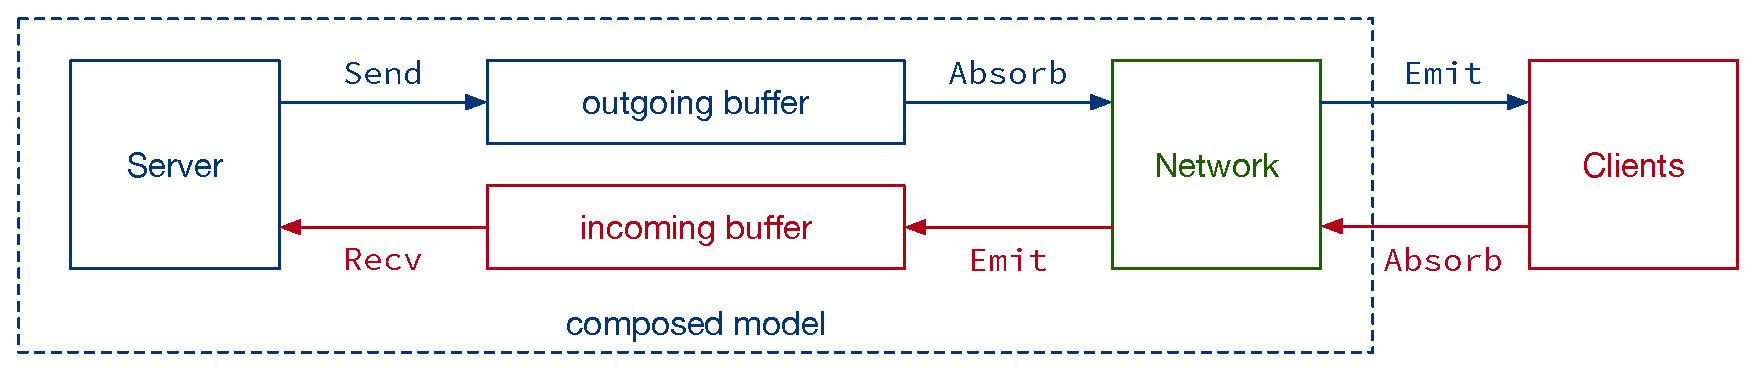
\includegraphics[width=\textwidth]{figures/net-compose}
  \caption{Network composition architecture.}
  \label{fig:net-compose}
\end{figure}

To handle the asynchronicity among the server and network events, I insert
message buffers between them.  As shown in \autoref{fig:net-compose}, the {\em
  incoming buffer} stores the packets emitted by the network but not yet
consumed by the server's \ilc{Recv} events, and the {\em outgoing buffer} stores
the packets sent by the server but not yet absorbed by the network.

\begin{figure}
\begin{lstlisting}[numbers=left]
CoFixpoint compose {E} (srv: itree smE void)          (* server  model *)
           (net  : itree (netE +' nondetE) void)      (* network model *)
           (bi bo: list packet)       (* incoming and outgoing buffers *)
           : itree (netE +' nondetE +' E) void :=
  let step_net :=%\label{line:step-net-def}%
    match net with
    | Impure Absorb knet =>
      match bo with
      | pkt::bo' => compose srv (knet pkt) bi bo'%\label{line:net-absorb}%
      | []       => pkt <- trigger Absorb;;%\label{line:client-send}%
                    compose srv (knet pkt) bi bo
      end
    | Impure (Emit pkt) knet =>%\label{line:net-emit}%
      if toServer pkt
      then compose srv (knet tt) (bi++[pkt]) bo%\label{line:srv-incoming}%
      else trigger (Emit pkt);;%\label{line:net-send}%
           compose srv (knet tt) bi bo
    | Impure Or knet => b <- trigger Or;;
                      compose srv (knet b) bi bo
    | Pure vd => match vd in void with end
    end
  in
  match srv with
  | Impure Recv ksrv =>%\label{line:srv-recv}%
    match bi with
    | pkt::bi' => compose (ksrv pkt) net bi' bo%\label{line:srv-consume}%
    | [] => step_net%\label{line:step-net}%
    end
  | Impure (Send pkt) ksrv =>%\label{line:srv-send}%
    compose (ksrv tt) net bi (bo++[pkt])
  | Impure e ksrv =>        (* other events performed by the server *)
    r <- trigger e;; compose (ksrv r) net bi bo
  | Pure vd => match vd in void with end
  end.
\end{lstlisting}
\vspace*{1em}
\caption[Network composition algorithm.]{Network composition algorithm.  When the
  server wants to send a packet in \autoref{line:srv-send}, the packet is
  appended to the outgoing buffer until absorbed by the network
  in \autoref{line:net-absorb}, and eventually emitted to the client
  in \autoref{line:net-send}.  Conversely, a packet sent by the client is
  absorbed by the network in \autoref{line:client-send}, emitted to the server's
  incoming buffer in \autoref{line:srv-incoming}, until the server consumes it
  in \autoref{line:srv-consume}.}
\label{fig:net-compose-code}
\end{figure}

The server and the clients are the opposite ends of the network.  Each packet
has routing fields that indicate its source and destination.  When the network
emits a packet, we need to determine whether the packet is emitted to the
server's incoming buffer or to the clients, by inspecting its destination:
\begin{coq}
  Definition toServer (p: packet) : bool :=
    if p.(Destination) is server_conn then true else false.
\end{coq}

Now we can define the composition algorithm formally, as shown in
\autoref{fig:net-compose-code}.  The function takes the symbolic server model
in \autoref{sec:symbolic-model} and the network model in \autoref{sec:net-tcp},
and yields a symbolic model of the server's behavior observable from across the
network.

The composition function analyzes the server and the network's behavior:
\begin{enumerate}
\item When the server wants to send a packet in \autoref{line:srv-send}, the
packet is appended to the outgoing buffer.
\item When the network wants to absorb a packet in \autoref{line:net-absorb},
it first checks whether the server has sent some packet to its outgoing buffer.
If yes, then the network absorbs the oldest packet in the buffer.  Otherwise, it
absorbs from the clients.
\item After absorbing some packets, when the network wants to emit a packet in
\autoref{line:net-emit}, the packet is either emitted to the client or appended
to the server's incoming buffer, based on its destination.
\item When the server wants to receive a packet in \autoref{line:srv-recv},
it first checks whether the network has emitted some packet to the incoming
buffer.  If yes, then the server takes the oldest packet in the buffer.
Otherwise, it waits for the network model to emit one.
\end{enumerate}

Note that this algorithm schedules the server at a higher priority than the
network model.  The composed model only steps into the network model when the
server is starved in \autoref{line:step-net}, by calling the \ilc{step_net}
process defined in \autoref{line:step-net-def}.  This design is to avoid
divergence of the derived tester program, which I'll further explain in
\autoref{sec:backtrack}.

By composing the server and network models, we get a symbolic model that may
send and receive packets asynchronously, as opposed to the server model that
processes one request at a time.  Dualizing this asynchronous symbolic model
results in an asynchronous tester model that may send multiple requests
simultaneously rather than waiting for previous responses.  Next I'll show how
to execute the tester's ITree model against the SUT.
